\chapter{绪论}
水声传感器网络(UnderWater Acoustic Sensor Networks, UWASN)指的是在一定的水下区域内,通过各种传感器获取信息,并对水下节点进行水声通信和组网,进而实现信息传输目的网络\cite{范光宇2015水声传感网络的媒体接入控制技术}。UWASN可用于海洋灾害预警预报、深海能源与资源开发、海洋环境监测、维护国家海洋安全等方面。


\section{研究背景}
移动水声传感网络由多个水下固定传感器节点和移动节点如UUV和AUV等组成,这些节点被布放在水下一个给定区域内,共同执行观测任务。图\ref{f1}是一个典型的水声传感器网络,AUV、固定结点和海面浮标之间可以相互通信,海面浮标和控制中心利用卫星通信\cite{noh2012mac}。
\begin{figure}[ht]
	\centering
	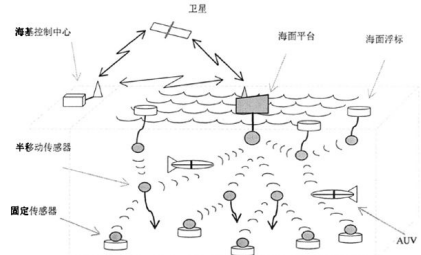
\includegraphics[scale=0.25]{figures/1.png}
	\caption{
		典型的水声传感网络
	}
	\label{f1}
\end{figure}

其中,搭载有各种设备的AUV/UUV可以在水下按特定轨迹航行,是水下传感网络中常用的移动平台。移动节点的加入为海洋立体观测提供了可能,扩大了网络的监控范围;同时移动节点可以对网络进行配置,如节点失效时,移动节点可以检测通信空洞并指导布放新节点,提高网络的稳健性。UWASN也可以为移动节点的导航提供支持,进行水下定位等。

\subsection{水声传感网络发展过程}
美国是最早开始研究水声传感网络的国家。1994年,美国伍兹霍尔海洋研究所(WHOI)\cite{freitag2005whoi}开发了第一代水声通信局域网(ALAN),该网络由一个海面浮标站和十几个1000m水深的海底节点构成,主要功能是将海底节点产生的数据发往水面站以及将水面站产生的控制信息发向海底节点。2005年WHOI用水声传感网络进行了海底地震探测实验。该网络由3个不同的水下传感器组成,每天向系在船上的浮标发送六次水声数据,这些浮标可通过卫星中继将数据转发到岸上。网络允许的最大上行传送速率是4kbps,每天可上传数据达1.4MB。

欧共体在MAST计划的支持下开展了一系列的水声通信网络研究,主要包括ACME,LOTUS、SWAN、ROBLINKS等子计划\cite{赵占伟2011水声通信网络}。其中ACME\cite{acar2006acmenet}是研究基于浅水网络的稳健通信和网络协议,网络中节点最小数为3,水深6-10米,节点之间的距离是200-2000米,最高数据率是lkbit/s。LOTUS主要是研究基于超浅水域的长距离通信设备,其中点对点之间的通信距离可达到10km,载波频率为8kHz,最高数据速率4kbit/s,该系统针对超浅水域中存在的强时变的混响干扰以及多用户干扰等问题进行了技术攻关。使用三维水听器阵列进行空间分集,同时对每个发送端进行匹配,目前该系统已经进行了两次海上试验。SWAN计划的目标是在浅海条件下建立通信仿真模型。研究各种无训练条件下MEMU阵列处理方法。ROBLINKS\cite{van2000roblinks}计划主要是研究浅海条件下,水深20-30m,距离大于10km的稳健通信项目,开发新的最佳相关信号处理算法是其研究重点,通过连续信道辨识技术,提高通信系统对周围环境变化的适应能力,并对算法进行海上验证。

中国在水声传感网络领域的研究起步较晚。主要研究机构有中科院声学所、哈尔滨工程大学、浙江大学、东南大学、厦门大学、、中国海洋大学、西北工业大学等。研究内容主要是低速率远程通信和高速率近程通信,同步技术以及组网技术等。

\subsection{水声传感网络协议栈}
水声传感网络按分层结构一般可以分为物理层、数据链路层和网络层\cite{赵占伟2011水声通信网络}。
\paragraph{物理层}
物理层负责数据的调制解调,把数字信息转换成能在水声信道中传输的声信号。在接收端检测被噪声及其他信道失真畸变的信号,并把信号恢复成原传送的数字信息。物理层面临的挑战是如何克服水声信道的恶劣条件,包括长传播时延、高延时抖动、窄带宽、高误码率等特点对信息传输带来的影响,如何对长延时网络进行同步,以及如何简化设计发送端和接收端来降低成本提高性能。水声网络物理层主要的技术有相干解调、非相干解调、正交频分复用(Orthogonal Frequency Division Multiplexing,OFDM)和多输入多输入(Multiple Input Multiple Output,MIMO)技术。
\paragraph{数据链路层}
数据链路层负责将来自网络层的指令和数据封装成帧,帧是数据链路层固有的结构,它含有足够的控制信息,保证数据可以通过网络成功发送到目的节点。数据链路层还负责把从物理层接收到的二进制数据重新组装成帧。数据链路层协议面临的挑战是
如何使每个传感器节点都可以公平、有效得分享带宽资源,使网络获得尽可能高的吞吐量,同时使占有时延尽可能小,消耗能量尽可能少。MAC协议应用在这一层中。
\paragraph{网络层}
网络层的任务是选择合适的路由信息,确定和分发源节点和目的节点之间的路由搜索及维护信息。其功能包括邻居发现、分组路由、拥塞控制和网络互联等。网络层面临的挑战是
如何使路由查找时间尽可能短,减少引入的额外时延,如何使维护路由的控制信息应尽量少,如何避免拥塞并提供QoS保证。



\subsection{面临的问题}
要达到可靠高效的端到端传输面临着很多挑战,主要体现在以下几个方面:

(1)水声信道可用带宽一般只有几kHz到几十 kHz,且随着通信距离的增加而减少,通信速率低。

(2)水声信道存在复杂的时、空、频变及强多途、高噪声、Doppler效应等因素,误码率高且中断概率大。

(3)声波传播速度低,传播时延长。

(4)节点存在移动性,由于水流等环境因素影响以及搭载平台的关系,大多数水下传感器节点存在着不同程度的移动,节点的移动导致传播时延变化。

(4)网络拓扑高动态:由于海洋环境恶劣,水下节点较容易出现故障或短暂失效,导致了网络节点不稳定的邻居关系。

(5)网络节点能量受限:水声节点长期工作在水下,充电困难且费用高,是能量资源严重受限的系统,节点之间相对更远的距离,以及为了弥补信道损耗,接收器对信号做了更复杂的处理都大大增加了能量的消耗。水声单位能量资源能传输的数据量比陆地无线通信低3个数量级。

水声网络大多是面向特定任务应用场景,以满足预定需求为设计目标,既可单独组网,也可与水下有线网络混合组网。预定任务的不同需求,如节点移动性、节点布署密度、网络覆盖范围、网络生命周期、网络传输可靠性等,将导致水声网络的不同设计\cite{徐文2016海洋信息获取}。

\section{研究内容}
本研究针对由移动节点和水下固定传感器组成的小规模单跳网络,结合海洋信息采集中对移动水声传感网络的各类需求,从设计移动节点接入机制、降低整体传输时延等方面入手,进行了如下的研究:
\begin{itemize}
	\item 针对移动节点接入固定节点网络,单向采集固定节点数据的场景,设计移动节点的接入和离开机制。移动节点加入固定节点网络时,需要发送广播包通知固定节点进行数据传输。充分利用广播包信息以及降低移动节点接入离开机制的开销,是流程设计时的重点。
	\item 针对移动水声网络的不可靠性高的特性,设计数据帧重传机制。数据重传时从握手机制开始重传带来的时间和能耗开销太大,在第一次传输时给数据帧重传设计专有的机制是必要的。
	\item 针对网络负载较大时控制帧冲突概率较高的问题,设计自适应负载变化的数据帧发送机制。协议设计时,低负载网络和高负载网络的优化方向各不相同,因此能够自适应负载变化的协议可以更好得应对各种网络场景。
\end{itemize}

\section{章节安排}
本文的章节安排如下,

第一章绪论,主要介绍了水声传感网络的概念、发展历史和体系结构,说明了本文的研究背景和应用场景,提出了研究需要解决的问题,在此基础上引出了研究的主要内容。

第二章介绍了水声网络MAC协议的分类,分析了移动水声网络MAC协议研究的国内外现状。

第三章重点介绍了两个竞争型水声传感网络MAC协议,UWALOHA和SFAMA。

第四章针对有移动节点接入的单跳水声网络,提出了基于竞争的LACC-M协议。首先介绍了CSMA/CA协议的基本原理。然后,重点介绍了移动节点的接入离开机制、数据帧重传机制和不同网络负载情况下的数据帧发送机制。

第五章介绍了提出的LACC-M协议的具体实现流程,并对协议性能进行了理论计算。

第六章介绍了仿真软件NS2和仿真平台Aqua-Sim,给出了四个网络性能指标,分析了仿真实验的结果。

\endinput